\section{Sam Windrider}\label{sam-windrider}

Tags: NPC, Quartiermastro Creatore: Lorenzo

\section{Sam Windrider}\label{sam-windrider-1}

\begin{center}\rule{0.5\linewidth}{0.5pt}\end{center}

\begin{figure}
\centering
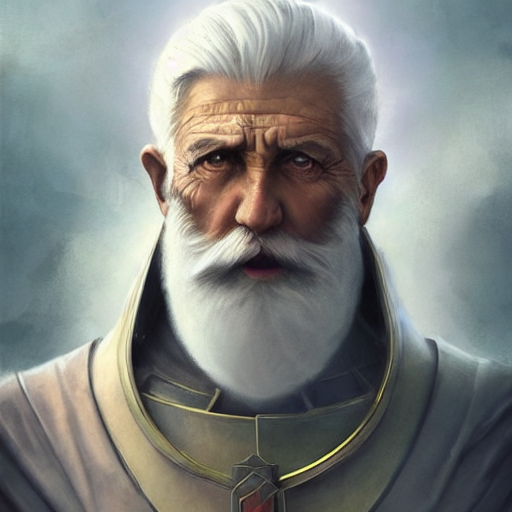
\includegraphics{Sam_Windrider.png}
\caption{Sam Windrider.png}
\end{figure}

Informazioni Generali

Età: 78

Anno di nascita: 1945

Paese di nascita: Kos

Razza: Umano

Relazioni:

Alleati: Gilda dei Protettori, Ordine dei Paladini di San Francesco.

Nemesi: Setta del Sangue

Possedimenti importanti:

Ruolo: Gran Custode del Tempio

\begin{center}\rule{0.5\linewidth}{0.5pt}\end{center}

\subsection{1. Descrizione Generale}\label{descrizione-generale}

\begin{center}\rule{0.5\linewidth}{0.5pt}\end{center}

Sam ha ancora un portamento fiero, nonostante la sua età avanzata. La
sua postura è leggermente curva, ma ciò non diminuisce la sua presenza
imponente. Il suo viso rugoso e segnato dal tempo è illuminato da un
sorriso gentile, mentre i suoi occhi incavati e profondi sembrano
raccontare tutto il dolore che hanno visto nella loro lunga vita.
Nonostante l'età avanzata, cammina con passo fermo e ha occhi brillanti
di saggezza. Dopo la morte del figlio, Sam decise di deporre le armi e
di ritirarsi nel tempio di San Francesco. Non volendo più essere
coinvolto nella violenza del mondo esterno, dedicò il resto della sua
vita alla preghiera e alla meditazione. È il paladino capo del tempio di
San Francesco ed è sua premura occuparsi di ogni cosa: dal benessere dei
fedeli alla manutenzione della struttura. La sua presenza ispira
rispetto e calma a tutti coloro che si avvicinano a lui, e la sua
saggezza è ricercata da molti che cercano consiglio e conforto.

\subsection{2. Biografia}\label{biografia}

\begin{center}\rule{0.5\linewidth}{0.5pt}\end{center}

\subsection{3. Carriera}\label{carriera}

\begin{center}\rule{0.5\linewidth}{0.5pt}\end{center}

\subsection{4. Personalità}\label{personalituxe0}

\begin{center}\rule{0.5\linewidth}{0.5pt}\end{center}

\subsection{A. Coinvolgimenti in eventi
recenti}\label{a.-coinvolgimenti-in-eventi-recenti}

\begin{center}\rule{0.5\linewidth}{0.5pt}\end{center}

\href{Untitled\%20Database\%2011e31a90c4de4b4e8b6da34fd12f13e9.csv}{Untitled
Database}

\subsection{B. Aggiornamenti}\label{b.-aggiornamenti}

\begin{center}\rule{0.5\linewidth}{0.5pt}\end{center}

\href{Untitled\%20f91756bc0aea4e4ab43710d40315e574.csv}{}
